\documentclass{standalone}
\usepackage{tikz}
\usetikzlibrary{arrows.meta, positioning}

\begin{document}

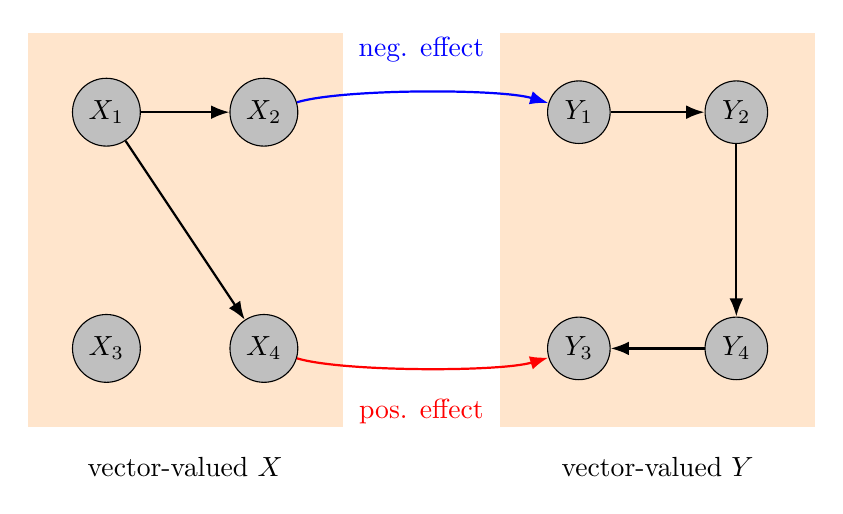
\begin{tikzpicture}[
    node distance=1cm and 1cm,
    dot/.style={circle, draw=black, fill=gray!50, minimum size=7mm},
    box/.style={rectangle, draw=none, fill=orange!20, minimum width=4cm, minimum height=5cm, rotate=0},
    arrow/.style={-{Latex}, thick},
    negEff/.style={arrow, blue},
    posEff/.style={arrow, red},
    inner/.style={arrow, black}
]

% Background boxes
\node[box, rotate=0] (Xbg) at (0,0) {};
\node[box, rotate=0] (Ybg) at (6,0) {};

% Nodes in X
\node[dot] (X1) at (-1,1.5) {$X_1$};
\node[dot] (X2) at (1,1.5) {$X_2$};
\node[dot] (X3) at (-1,-1.5) {$X_3$};
\node[dot] (X4) at (1,-1.5) {$X_4$};

% Nodes in Y
\node[dot] (Y1) at (5,1.5) {$Y_1$};
\node[dot] (Y2) at (7,1.5) {$Y_2$};
\node[dot] (Y3) at (5,-1.5) {$Y_3$};
\node[dot] (Y4) at (7,-1.5) {$Y_4$};

% Intra connections
\draw[inner] (X1) -- (X2);
\draw[inner] (X1) -- (X4);
\draw[inner] (Y1) -- (Y2);
\draw[inner] (Y2) -- (Y4);
\draw[inner] (Y4) -- (Y3);

% Inter connections
\draw[negEff] (X2) .. controls (2,1.8) and (4,1.8) .. (Y1);
\draw[posEff] (X4) .. controls (2,-1.8) and (4,-1.8) .. (Y3);

% Labels
\node at (0,-3) {vector-valued $\boldsymbol{X}$};
\node at (6,-3) {vector-valued $\boldsymbol{Y}$};
\node[blue] at (3,2.3) {neg. effect};
\node[red] at (3,-2.3) {pos. effect};

\end{tikzpicture}

\end{document}